Idealmente per tensioni \textit{gate-source} inferiori alla tensione di soglia il transistore MOSFET non lascia passare nessuna corrente di \textit{drain}, $I_D = 0$. Nella realtà questo non è vero, infatti sono presenti le cosiddette \textit{leakage current}, correnti di perdita, che possono variare a seconda della tipologia del dispositivo, NMOS o PMOS, o anche per la dimensione.
Queste correnti possono essere rilevanti o trascurabili a seconda dell'intensità; In figura \ref{fig:i_off_confronto}, confronti tra NMOS e PMOS delle correnti di perdita estratti per valori di $V_{GS} = -0.3V$ e $V_{DS} = 0.45V$\footnote{Per i PMOS si intendono $V_{SG} = -0.3V$ e $V_{SD} = 0.45V$}.

\paragraph*{Differenze di $\bm{I_{off}}$ tra NMOS e PMOS} Nella figura \ref{fig:i_off_confronto} la differenza tra i dispositivi a canale N e a canale P è molto evidente superati i $600Mrad$, soprattutto per il dispositivo $600-0.060$ \ref{sub@fig:i_off_confronto_600_60_e_180}, raggiungendo differenze all'ordine dei $\mu A$. Infatti, come già anticipato nella sezione \ref{cap1:ionizzazione}, i MOSFET a canale N sono soggetti alla creazione di transistor parassiti nella \textit{STI} che comportano un aumento della $I_{off}$.

\paragraph*{Differenze di $\bm{I_{off}}$ in dispositivi a dimensioni diverse} La corrente di \textit{drain} presenta una proporzionalità con le dimensioni del dispositivo, in particolare $I_{D} \propto \frac{W}{L}$. Osservando, ad esempio, la figura \ref{fig:i_off_confronto_600_60_e_180} si nota come la l'aumento della lunghezza, da $60 \text{ a } 180nm$ provoca un abbassamento della $I_{off}$, mentre a parità di $L$ e all'aumentare di $W$ si ha un aumento della corrente di perdita.

\paragraph*{Effetto della $\bm{\Delta V_{th}}$ a basse dosi sui NMOS} Come già riportato nella sezione \ref{cap1:ionizzazione}, e confermato dai dati nella sezione \ref{cap2:vth}, la variazione della tensione di soglia, nei dispositivi NMOS, inizialmente è negativa a basse dosi (circa $10Mrad$) e la riduzione della $V_{th}$ comporta un aumento della corrente \textit{drain-source} di perdita, in figura \ref{fig:i_off_confronto_bassi_dosaggi} vengono mostrati gli andamenti della $I_{off}$ per i dispositivi a larghezza $100\mu m$ con lunghezza $60 nm \text{ e } 180nm$ e per i dispositivi $W = 600\mu m$ e $L = 60 nm \text{ e } 180nm$, con un focus particolare sui bassi dosaggi di radiazioni ionizzanti.

\begin{figure}[h]

    \centering
    
    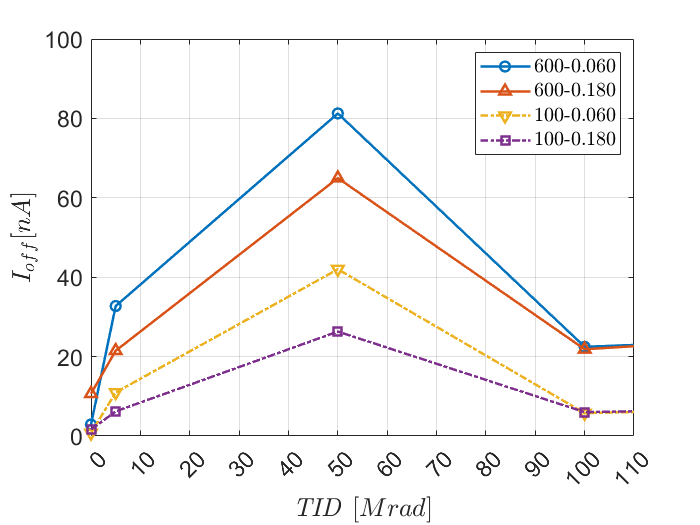
\includegraphics[width = 0.7 \linewidth ]{capitolo2/I_off/confornto_bassi_dosaggi/i_off_bassi_dosaggi.png}
    \caption[Confronto della $I_{off}$ di diversi dispositivi]{Confronto della $I_{off}$ di diversi dispositivi NMOS}
    \label{fig:i_off_confronto_bassi_dosaggi}
    
    \vspace{1cm}
    
    \centering
    \subfloat[
        \centering{Linea continua: $100-0.030$\\
        Linea tratteggiata: $100-0.060$}
    ]{
        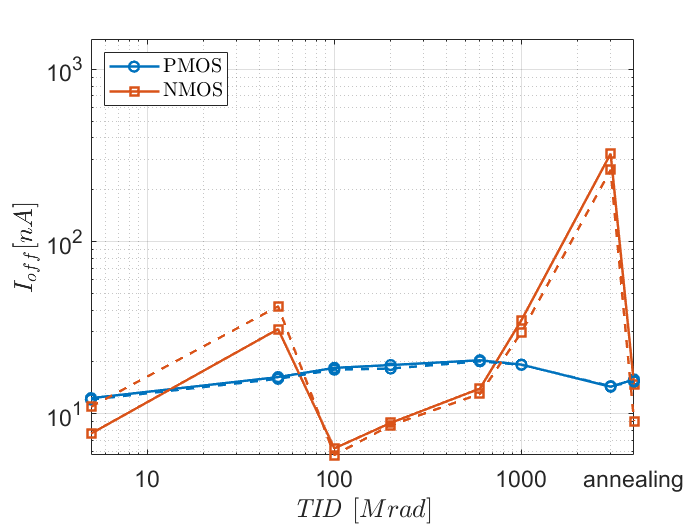
\includegraphics[width = 0.49 \linewidth]{capitolo2/I_off/confornto/I_off_confronto_NP_100-30_e_60.png}
        \label{fig:i_off_confronto_100_30_e_60}
    }
    \subfloat[
        \centering{Linea continua: $600-0.060$\\
        Linea tratteggiata: $600-0.180$}
    ]{
        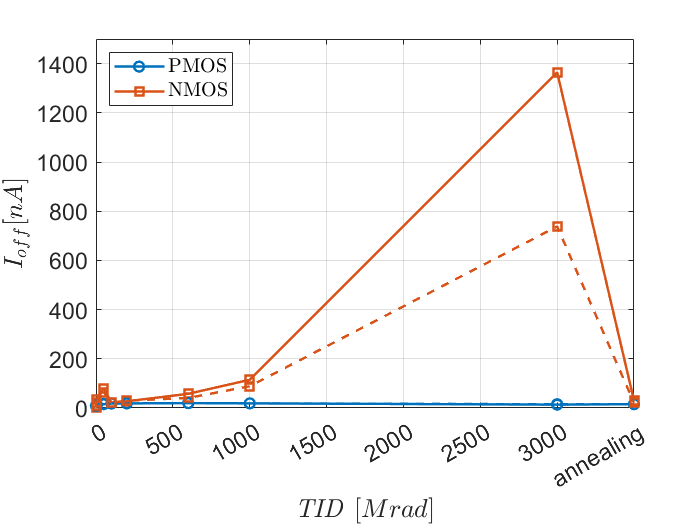
\includegraphics[width = 0.49 \linewidth]{capitolo2/I_off/confornto/I_off_confronto_NP_600-60_e_180.png}
        \label{fig:i_off_confronto_600_60_e_180}
    }

    \caption[Confronto \textit{leakage current} tra dispositivi]{Confronto \textit{leakage current} tra dispositivi NMOS e PMOS; a sinistra, figura \ref{sub@fig:i_off_confronto_100_30_e_60}, le larghezze $100\mu m$ mentre a figura \ref{sub@fig:i_off_confronto_600_60_e_180} le larghezze $600\mu m$.}
    \label{fig:i_off_confronto}
    

\end{figure}

\vspace{0.5cm}
Per concludere si riportano a figura \ref{fig:delta_i_off} i grafici delle variazioni della \textit{leakage current}, $\Delta I_{off}$, al variare della dose assorbita.

\clearpage

\begin{figure}[ht]
    
    \includegraphics[width = 0.49\linewidth]{capitolo2/I_off/NMOS/Delta_I_off_W_100_VDS_450_mV.png}
    \includegraphics[width = 0.49\linewidth]{capitolo2/I_off/PMOS/Delta_I_off_W_100_VDS_450_mV.png}\\
    \vspace{0.2cm}
    \includegraphics[width = 0.49\linewidth]{capitolo2/I_off/NMOS/Delta_I_off_W_200_VDS_450_mV.png}
    \includegraphics[width = 0.49\linewidth]{capitolo2/I_off/PMOS/Delta_I_off_W_200_VDS_450_mV.png}\\
    \vspace{0.2cm}
    \includegraphics[width = 0.49\linewidth]{capitolo2/I_off/NMOS/Delta_I_off_W_600_VDS_450_mV.png}
    \includegraphics[width = 0.49\linewidth]{capitolo2/I_off/PMOS/Delta_I_off_W_600_VDS_450_mV.png}
    
    \caption[$\Delta I_{off}$ al variare della dose assorbita]{Confronti della $\Delta I_{off}$ al variare della dose assorbita, NMOS (sinistra) e PMOS (destra). I dispositivi sono raggruppati per larghezza di canale.}
    \label{fig:delta_i_off}
\end{figure}

\FloatBarrier